El programa de línea de base del \LHC~ tenía el objetivo de producir los primeros resultados en la carrera 2010-2012 con el objetivo de una \href{https://es.wikipedia.org/wiki/Luminosidad}{luminosidad integrada} de al menos $1~fb^{-1} = 40~m^2$ para fines de 2011 y gracias a un rendimiento mejor de lo previsto se obtuvo más de $25~fb^{-1}$ en colisión de $pp$ a finales de 2012, más allá de cualquier expectativa. Después se alcanzó la energía de $13-14~TeV$ de centro de masa de energía en 2015.

Después de 2019, la ganancia estadística al ejecutar el acelerador sin un aumento considerable de luminosidad más allá de su valor de diseño fue más de la prevista. El tiempo de ejecución necesario para reducir a la mitad el error estadístico en las mediciones. Por lo tanto, para mantener el progreso científico y explorar su capacidad total, el \LHC ~ necesitará un aumento decisivo de su luminosidad. Por eso, cuando el Consejo del \CERN ~ adoptó la Estrategia Europea para la Física de Partículas en Bruselas el 30 de mayo de 2013, se acordó que su primera prioridad sería:

\begin{minipage}{0.9\linewidth}
\vspace{5pt}%margen superior de minipage
{\small }
\textit{``La máxima prioridad de Europa debería ser la explotación de todo el potencial del \LHC, incluido el actualización de alta luminosidad de la máquina y los detectores con el fin de recopilar diez veces más datos que en el diseño inicial, alrededor de 2030''}
\begin{flushright}
cita traducida de la referencia \cite{wells_upgraded_2015}
%(\citeauthor{Coulouris}, \citeyearNP{Coulouris}: 10)
\end{flushright}
\vspace{5pt}%margen inferior de la minipage
\end{minipage}

Además se reemplazarán los imanes triples internos (el responsable de exprimir el rayo en caso de colisión) y de todos los cambios de hardware necesarios para permitir una ambiciosa actualización de luminosidad. Con algunas de las modificaciones ya cumplidas en 2019 ($LS2$), esta nueva fase de la vida del \LHC ~ se ha denominado ``\LHC ~ de alta luminosidad'' (\textbf{HL-}\LHC) y tiene la aspiración de alcanzar el sorprendente umbral de $3000~fb^{-1}$ en 10-12 años, entregarando hasta la actualización aproximadamente $\backsim 300~fb^{-1}$ durante ese período (ver Fig. \ref{cms_actualiza}).


\begin{figure}[h!]
\centering
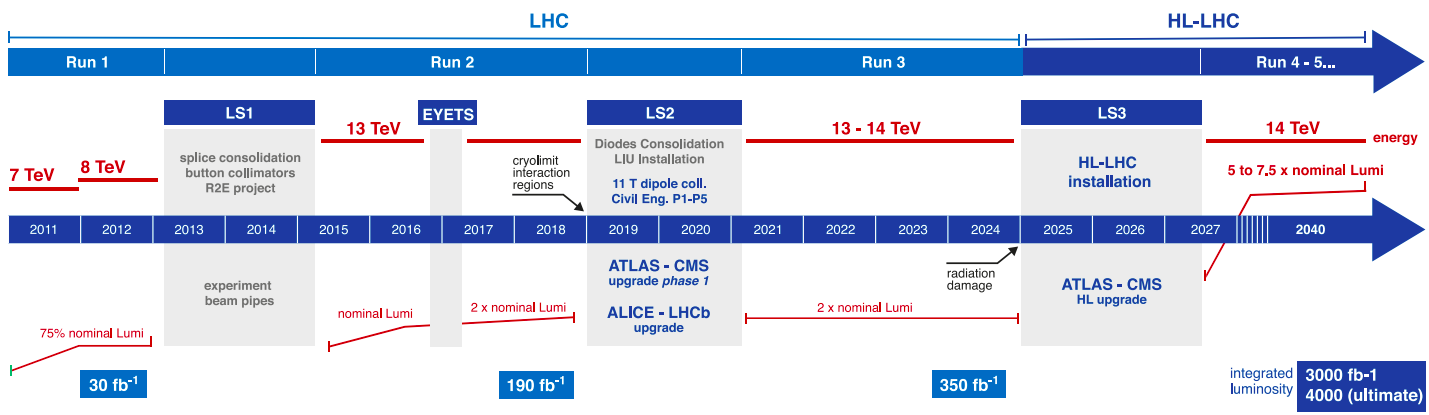
\includegraphics[width=1\textwidth]{Analisis_y_Resultados/imagenes/CMS_upgrade.png}
\caption{Plan de actualización del experimento \LHC. Pagina de origen: \url{https://hilumilhc.web.cern.ch/content/hl-lhc-project}.}
\label{cms_actualiza}
\end{figure}

Con la actualización del \LHC ~se espera aumentar los conocimiento más allá del Modelo Estándar y su bosón de Higgs, siendo sus apuestas a la misteriosa materia oscura, con la teoría de la supersimetría. Pero para lograr actualizar una maquinaria tan compleja a tan gran escala se planifica una década en completarse. El proceso depende de una serie de tecnologías innovadoras que el proyecto \textbf{HL-}\LHC ~ está explorando. Esta extraordinaria empresa técnica dependerá de una combinación de imanes superconductores $11-12~T$ de vanguardia, cavidades de radiofrecuencia superconductoras compactas y ultraprecisas para la rotación del haz, así como enlaces superconductores de alta potencia de $100 ~m$ de largo con disipación de energía cero. Además, las altas luminosidades generarán nuevas demandas de vacío, criogenia y protección de la máquina, y requerirán nuevos conceptos para la colimación y el diagnóstico, modelado avanzado para el haz intenso y nuevos esquemas de cruce del haz para maximizar la salida física de las colisiones.



